\documentclass[tikz,border=10pt]{standalone}
\usepackage{pgfplots}
\pgfplotsset{compat=1.18}
\usepackage{amsmath}
\usepackage{amssymb}
\definecolor{mantis}{RGB}{0, 105, 62}
\begin{document}
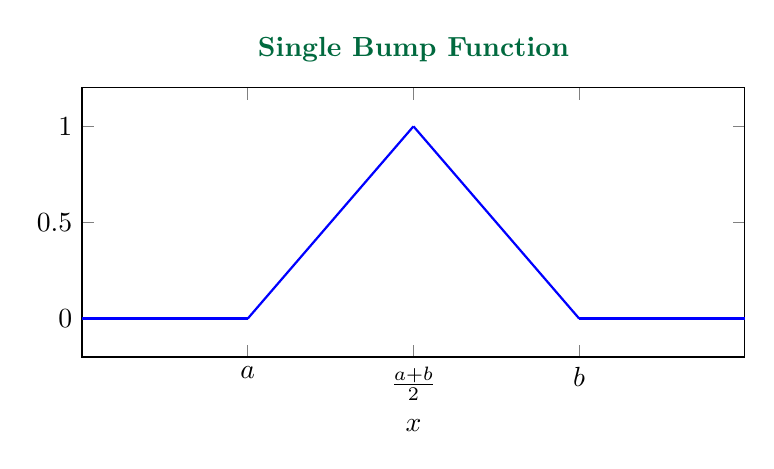
\begin{tikzpicture}
\begin{axis}[
    width=10cm,
    height=5cm,
    xlabel={$x$},
    xmin=-0.5, xmax=3.5,
    ymin=-0.2, ymax=1.2,
    xtick={0.5, 1.5, 2.5},
    xticklabels={$a$, $\frac{a+b}{2}$, $b$},
    title={\textbf{Single Bump Function}},
    title style={font=\bfseries\color{mantis}},
]
\addplot[domain=-0.5:0.5, samples=20, color=blue, thick] {0};
\addplot[domain=0.5:1.5, samples=20, color=blue, thick] {x-0.5};
\addplot[domain=1.5:2.5, samples=20, color=blue, thick] {2.5-x};
\addplot[domain=2.5:3.5, samples=20, color=blue, thick] {0};
\end{axis}
\end{tikzpicture}
\end{document}
